\chapter{Comparative Analysis of Weather Masking}
\section{Setup}
\subsection{Dataset}
Requirements for the Dataset on this project:
\begin{itemize}
    \item Large Dataset: The dataset should be extensive to cover a wide range of scenarios.
    \item Multiple Weather Conditions: It should include data from various weather conditions to ensure robustness.
\end{itemize}
Dataset Recommendation: A dataset that meets these requirements is BOARS.\\
This dataset offers several benefits:
\begin{itemize}
    \item Comprehensive Toolkit: A toolkit is provided to assist with using the dataset.
    \item Weather Diversity: The dataset includes data from multiple weather conditions.
\end{itemize}
However it has some drawbacks:
\begin{itemize}
    \item Linux-Only Toolkit: The toolkit is compatible only with Linux devices.
    \item All dataset Requirements: The toolkit requires radar, LiDAR, and camera data to function.
    \item Large File Sizes: Each part of the dataset is quite large, with each section being approximately 100GB, making it difficult to download.
    \item Poor Documentation: The documentation for each section of the dataset is inadequate.
    \item Third-Party Software: Downloading parts of the dataset requires installing third-party software from Amazon.
\end{itemize}

\subsection{Model}

\subsubsection{SPADE}
The SPADE (Spatially-Adaptive Denormalization) model from NVIDIA is a groundbreaking approach for semantic image synthesis. Introduced in 2019, SPADE addresses the limitations of traditional normalization techniques that often wash away semantic information. Instead of directly feeding the semantic layout into the network, SPADE uses the layout to modulate the activations in normalization layers through a spatially-adaptive, learned transformation. This method allows for the generation of photorealistic images that align closely with the input semantic maps. SPADE has demonstrated superior performance on challenging datasets like COCO-Stuff and Cityscapes, enabling users to control the style and content of the synthesized images effectively.
\\ I selected SPADE for this project. SPADE gets two images Segmentation and Edge. its output is a single RGB image.
\subsubsection{Pix2Pix}
The pix2pix model, developed by UC Berkeley, uses a conditional Generative Adversarial Network (cGAN) for image-to-image translation tasks like converting sketches to photos. It consists of a Generator and a Discriminator to create and evaluate images. For my project, I used the `pytorch-CycleGAN-and-pix2pix` implementation, which simplifies training and testing these models for high-quality image synthesis.
\section{Implementation}
\subsection{Dataset}
\subsubsection{Train dataset}
I randomly selected images from the dataset and applied rotations to some samples to augment the dataset size. The images were resized to 1888x1576 pixels and converted from PNG to JPG format. Both the mask and cloud point retained the same dimensions. Initially, the dataset contained 129,000 items when using SPADE. However, after the first training, I resampled the dataset to 1/10th of its original size, resulting in 12,900 items.

\begin{table}[h]
    \centering
    \begin{tabular}{|l|c|c|c|c|c|c|c|}
        \hline
        Condition  & Snow    & Raining & Sun     & Clouds  & Snowing & Overcast \\
        \hline
        Percentage & 17.15\% & 16.62\% & 19.14\% & 15.54\% & 15.67\% & 15.88\%  \\
        \hline
    \end{tabular}
    \caption{the precntge of each weather.}
\end{table}
The percentage of each weather condition remain the same number after the decreasing of sample size.
\\
The base dataset all mask are same and they are 0 grayscale, On the other hand, the dataset for each weather condition includes spatial image masks with varying grayscale values, spaced at intervals of 30 degrees.
\subsubsection{Validation set}
I used 120 images from BOARS. Every weather condition has the same precntage 16.67\%.
\subsection{SPADE}
I changed the model to accept two images. A camera image and a weather mask image and the output of it be a cloud point image.
\\
I modified the model to concatenate the camera image with the paired weather mask in the similar way as the original SPADE works with Segmentation and Edge images, resulting in a 4-dimensional tensor.
This increase in dimensions necessitates modifications to the convolution layers.
\subsection{Pix2Pix}
The original Pix2Pix get single image however I modified the model to accept two input images: a camera image and a weather mask image. The output of the model is a cloud point image.
I modified the model to concatenate the camera image with the paired weather mask in the
similar way as the original SPADE works with Segmentation and Edge images, resulting in a 4-
dimensional tensor. However, this model requires less modifications in convolution layers paramenter because many of them come from the option.

\section{Result}
I trained the models using two datasets. The first was a base dataset that applied the same weather mask for every weather condition, serving as a baseline for comparison. The second dataset included weather conditions where each condition had a unique spatial mask.

Initially, the SPADE model experienced underfitting for the first 30 epochs. However, as the number of epochs increased, this issue began to diminish.

While there was no significant difference in performance between the base and weather conditions models regarding weather conditions, a notable difference emerged in their ability to predict distorted camera images. The models trained with the spatial masks showed improved accuracy in handling these distortions.
\begin{figure}[!ht]
    \begin{minipage}[t]{.24\linewidth}
        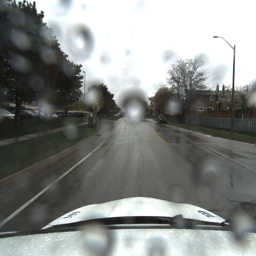
\includegraphics[width=\linewidth]{imgs/base/camera.png}
    \end{minipage}\hfill
    \begin{minipage}[t]{.24\linewidth}
        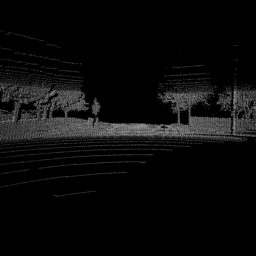
\includegraphics[width=\linewidth]{imgs/base/ground.png}
        \hbox{ground}
    \end{minipage}
    \begin{minipage}[t]{.24\linewidth}
        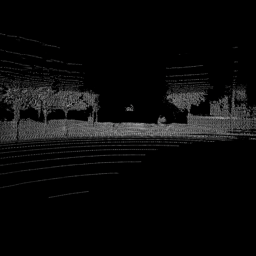
\includegraphics[width=\linewidth]{imgs/base/same.png}
        \hbox{The same mask}
    \end{minipage}
    \begin{minipage}[t]{.24\linewidth}
        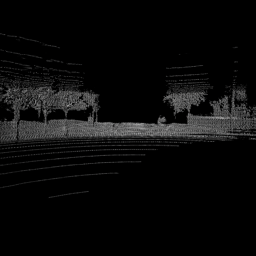
\includegraphics[width=\linewidth]{imgs/base/weathermasl.png}
        \hbox{Spatial weather mask}
    \end{minipage}
    \caption{A item of validation set which camera image be distorted}
    \label{img:result-camera}
\end{figure}

\begin{table}
    \centering
    \begin{tabular}{l c c}
        \hline
        Condition  & Same Mask    & Spatial weather mask \\
        \hline
        L1 loss & 5.4234 & 5.3506 \\
        \hline
    \end{tabular}
    \caption{The L1 loss for camera image distorted}
    \label{table:result-l1}
\end{table}
The table \ref{table:result-l1} shows the L1 loss of the image \ref{img:result-camera}. Nevertheless, the L1 loss between is similar in other conditions.